% Source: graduate-coursework/Sp26/CSCE763/Course_Assignments/Project/project_proposal.tex
% Description: Morphological detection pipeline. Structuring element operations remove noise before connected component extraction.

\documentclass[border=4pt]{standalone}
\usepackage{amsmath}
\usepackage{amssymb}
\usepackage{graphicx}
\usepackage{tikz}
\usepackage{xcolor}
\usetikzlibrary{positioning, arrows.meta, calc, fit, backgrounds, decorations.pathreplacing}

\definecolor{USC_Garnet}{HTML}{73000A}
\definecolor{USC_Black10}{HTML}{ECECEC}
\definecolor{USC_Black70}{HTML}{5C5C5C}
\definecolor{USC_Congaree}{HTML}{1F414D}

\begin{document}
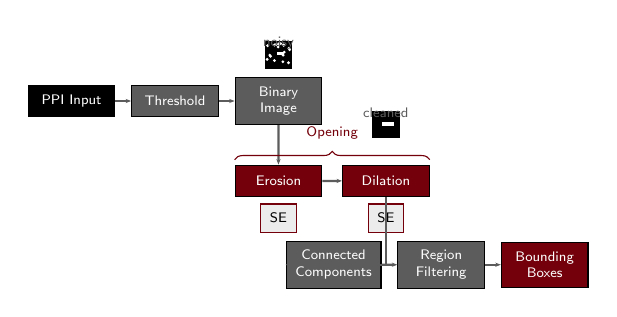
\begin{tikzpicture}[scale=0.78, every node/.style={font=\sffamily\tiny},
  block/.style={draw, fill=#1, text=white, minimum height=0.4cm,
    minimum width=1.1cm, font=\sffamily\tiny, align=center},
  block/.default={USC_Black70},
  arr/.style={-{Stealth[length=2pt]}, thick, USC_Black70},
  sebox/.style={draw=USC_Garnet, fill=USC_Black10, minimum height=0.28cm,
    minimum width=0.28cm, font=\sffamily\tiny}
]
  % Row 1
  \node[block=black] (input) {PPI Input};
  \node[block=USC_Black70, right=0.2cm of input] (otsu) {Threshold};
  \node[block=USC_Black70, right=0.2cm of otsu] (bin) {Binary\\Image};

  % Row 2 (below, shifted right)
  \node[block=USC_Garnet, below=0.5cm of bin] (ero) {Erosion};
  \node[sebox, below=0.08cm of ero] (se1) {\tiny SE};
  \node[block=USC_Garnet, right=0.25cm of ero] (dil) {Dilation};
  \node[sebox, below=0.08cm of dil] (se2) {\tiny SE};

  % Row 3 (below row 2)
  \node[block=USC_Black70, below=0.55cm of ero, xshift=0.7cm] (cc) {Connected\\Components};
  \node[block=USC_Black70, right=0.2cm of cc] (filt) {Region\\Filtering};
  \node[block=USC_Garnet, right=0.2cm of filt] (bbox) {Bounding\\Boxes};

  % Arrows row 1
  \draw[arr] (input) -- (otsu);
  \draw[arr] (otsu) -- (bin);
  % Arrow down to erosion
  \draw[arr] (bin.south) -- (ero.north);
  \draw[arr] (ero) -- (dil);
  % Opening brace over erosion+dilation pair
  \draw[decorate, decoration={brace, amplitude=3pt}, USC_Garnet]
    ([yshift=0.08cm]ero.north west) -- ([yshift=0.08cm]dil.north east)
    node[midway, above=4pt, USC_Garnet, font=\sffamily\tiny] {Opening};
  % Arrow down to CC
  \draw[arr] (dil.south) |- (cc.west);
  \draw[arr] (cc) -- (filt);
  \draw[arr] (filt) -- (bbox);

  % Illustrative before/after mini-squares
  \node[anchor=south, inner sep=0pt] at ($(bin.north)+(0,0.12)$) {%
    \tikz{
      \fill[black] (0,0) rectangle (0.35,0.35);
      \pgfmathsetseed{99}
      \foreach \i in {1,...,18} {
        \pgfmathparse{rnd*0.3+0.025}\let\px\pgfmathresult
        \pgfmathparse{rnd*0.3+0.025}\let\py\pgfmathresult
        \fill[white] (\px,\py) circle (0.02);
      }
      \fill[white] (0.15,0.18) rectangle (0.25,0.22);
    }%
  };
  \node[anchor=south, inner sep=0pt] at ($(dil.north)+(0,0.42)$) {%
    \tikz{
      \fill[black] (0,0) rectangle (0.35,0.35);
      \fill[white] (0.12,0.15) rectangle (0.28,0.21);
    }%
  };
  \node[USC_Black70, font=\sffamily\tiny] at ($(bin.north)+(0,0.55)$) {noisy};
  \node[USC_Black70, font=\sffamily\tiny] at ($(dil.north)+(0,0.85)$) {cleaned};
\end{tikzpicture}
\end{document}
